\chapter{Komunikacja w układzie}

Przesyłanie danych pomiędzy czujnikami a stacją główną (mikrokomputerem) jest najistotniejszą częścią całego układu. System pomiarów, po poprawnym, sprzętowym podłączeniu każdego z podzespołów, należy następnie skomunikować. Urządzenia pomiarowe wraz z głównym komputerem można komunikować poprzez interfejsy cyfrowe zaimplementowane w danym urządzeniu. Mikrokomputer BeagleBone Black obsługuje kilka interfejsów komunikacji: SPI, $\mathrm{I^{2}C}$, 1-Wire, CAN, UART. Możliwa jest również łączność poprzez zwykłe porty GPIO (General Purpose Input/Output). W układzie pomiarowym zastosowane zostały interfejsy $\mathrm{I^{2}C}$ oraz GPIO.

\section{Magistrala szeregowa $\mathbf{I^{2}C}$}
Magistrala jest to układ linii, po których przekazywane są wszystkie informacje pomiędzy podłączonymi do niej urządzeniami, np. komputerem, czujnikiem, regulatorem itp. Zasada działania magistrali opiera się na uzyskiwaniu oraz nadawaniu współpracującym częściom uprawnień do transmisji danych w danej jednostce czasu. W jednej chwili, w magistrali może działać tylko jedno urządzenie nadające oraz dowolna liczba odbiorców. Systemy o budowie opartej na magistrali są łatwo modyfikowalne oraz rozszerzalne, w prosty sposób można dołączyć lub odłączyć elementy systemu.
Dane przesyłane na dużą odległość najlepiej jest przekazywać transmisją szeregową, na krótsze odległości, przesyłanie równoległe oraz szeregowe daje podobne rezultaty.
Bity oraz całe słowa w tej komunikacji przesyłane są jeden po drugim. Przy takim sposobie łączenia się wystarczą tylko dwa przewody łączące odbiorcę z urządzeniem nadającym. 

Przykład urządzenia w magistrali szeregowej został przedstawiony na  rysunku \ref{fig:magistrala}.
\begin{figure}[h]
\centering
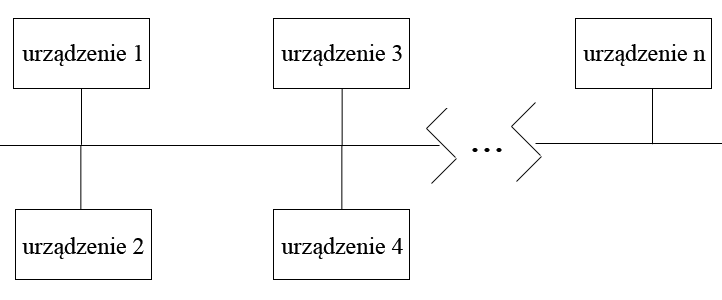
\includegraphics[scale=0.5]{magistrala}
\caption{Schemat magistrali szeregowej}
\label{fig:magistrala}
\end{figure}

Jak widać na załączonym schemacie, można podłączyć do magistrali wiele urządzeń. Wszystkie są podłączone do jednej lini danych, na której odbywa się komunikacja. To właśnie przez nią przesyłane są wszystkie dane pomiędzy elementami magistrali.


Nazwa magistrala szeregowej $\mathrm{I^{2}C}$ jest akronimem od Inter-Intergrated Circuit. Standard został opracowany w latach osiemdziesiątych przez firmę Philips.

Jest ona bardzo często wykorzystywana w układach mikroprocesorowych, w sterownikach wyświetlaczy LCD, można ją stosować do sterowania pamięci RAM, EPROM, układami I/O.

Zaletami magistrali $\mathrm{I^{2}C}$ są niewątpliwie takie właściwości jak:

\begin{itemize}
\setlength{\itemsep}{2pt} 
\setlength{\parskip}{2pt} 
\setlength{\parsep}{2pt}
\item odporność na zakłócenia zewnętrzne
\item części układu mogą być dodawane do niego lub wyłączane bez ingerencji w pozostały układ połączeń wcześniej stworzonych
\item połączenie na magistrali składają się tylko z dwóch przewodów, przez co ich ogólna liczba jest minimalizowana
\item wykrywanie błędów jest proste i łatwe do analizy
\item na magistrali może znajdować się wiele urządzeń typu master, umożliwiając kontrolę gotowych układów przez zewnętrzny komputer
\end{itemize}


Magistrala $\mathrm{I^{2}C}$ posiada dwie dwukierunkowe linie: dane są przesyłane przez Serial Data (SDA), natomiast sygnał zegara na Serial Clock (SCL).


Rysunek \ref{fig:i2c} prezentuje proces przesyłu danych przez magistralę $\mathrm{I^{2}C}$. Gdy nikt nie nadaje, linia zegara - SCL oraz danych - SDA są cały czas w stanie wysokim. W trakcie rozpoczęcia nadawania SCL ma stan wysoki, natomiast linia danych ma zbocze opadające. Po wysłaniu sygnału startu wysyłany jest z każdym taktem zegara bitowo adres urządzenia, z którym nastąpi komunikacja. Po wysłaniu 7 bitów adresu, wysyłany jest bit oznaczający, czy ma nastąpić pisanie czy czytanie z urządzenia slave. Kiedy podrzędna część układu rozpozna, że do niego jest adresowane zapytanie, w takcie dziewiątego bitu wysyła sygnał potwierdzenia przyjęcia dyspozycji. Taka sekwencja wysyłania danych jest powtarzana do momentu pojawienia się sygnału wysokiego na linii zegara oraz zbocza narastającego na linii danych. Od tego momentu magistrala znowu jest wolna i w dowolnej chwili dowolne urządzenie może zacząć nadawać, aby rozpocząć nową transmisję danych wystarczy powtórzyć powyższą sekwencję kroków.

\begin{figure}[h]
\centering
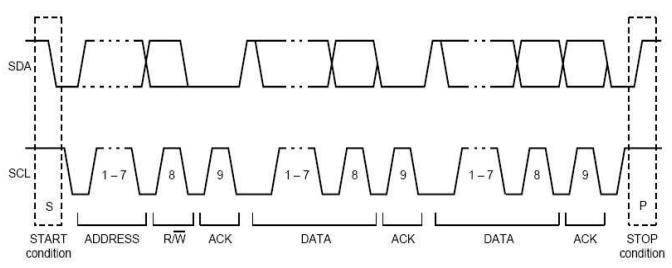
\includegraphics[scale=0.8]{i2c}
\caption{Wysyłanie danych poprzez magistralę $\mathrm{I^{2}C}$}
\label{fig:i2c}
\end{figure}

\section{Komunikacja z wykorzystaniem GPIO}
Porty GPIO są binarnymi złączami, które mogą służyć zarówno za wyjście dyskretne, jak i wejście. Ich kierunek jest zazwyczaj konfigurowalny i może być zmieniany w dowolnej chwile. Wejścia/wyjścia są kodowane poprzez odpowiednie napięcie na złączu.

Komunikacja mikrokontrolera oraz urządzeń peryferyjnych, przy użyciu GPIO odbywa się poprzez odpowiednie ustawianie wartości na wyjściu, tak aby drugie urządzenie mogło tą wartość odczytac i przeanalizować. Odpowiedź odbywa się najczęściej przy użyciu tego samego pinu, aby taka funkcjonalność zadziałała musi nastąpić zmiana kierunków pinu w obu częściach układu na przeciwny.
